\documentclass[a4paper,12pt,oneside,final]{extarticle}
\usepackage[top=2cm, bottom=2cm, left=3cm, right=1cm]{geometry}
\usepackage{scrextend}

\usepackage{fontspec}  
\usepackage{polyglossia}

\usepackage{tempora}
\setmainfont{tempora}
\setmainlanguage{russian} 
\setotherlanguages{english,ukrainian}


\frenchspacing

% Lists
\usepackage{enumitem}
\renewcommand\labelitemi{--}
\renewcommand\labelenumi{\arabic*}
\setlist[description]{noitemsep,style=multiline,leftmargin=2.5cm}
\setlist[itemize]{noitemsep, topsep=0pt}
\setlist[enumerate]{noitemsep, topsep=0pt}

\usepackage{titlesec}
\newcommand{\sectionbreak}{\clearpage}

\usepackage{hyperref} % make refs clickable
\usepackage{float}
\usepackage{pgfplots}
\usepackage{graphicx}
\usepackage{multirow}
\usepackage{amssymb,amsfonts,amsmath,amsthm}
\usepackage{csquotes}
\usepackage{xstring}
\usepackage{tabularx}

\numberwithin{equation}{section}

\usepackage{listings}
\lstset{basicstyle=\footnotesize\ttfamily,breaklines=true}
\lstset{language=Matlab}

\makeatletter
\def\maxwidth#1{\ifdim\Gin@nat@width>#1 #1\else\Gin@nat@width\fi}
\makeatother

\begin{document}
\title{Основы управление развитием организации}
\maketitle
\tableofcontents

%
% section 1
%
\section{Модуль I}
\subsection{Понятие и сущность управления}

\subsection{Управление и менеджеры}

\subsection{Развитие теории и практики управления. Современная система взглядов на управление}

\subsection{Определение <<организационная система>>. Организационные системы как системы междисциплинарной природы}

\subsection{Внутренняя и внешняя среда организационной системы}
Внутренняя среда организационной системы --- это ее организационное строение и ситуационные факторы внутри нее (внутренние переменные).
К основным переменным относятся: структура, цели, задачи, технологии и люди.

Производство --- это средства и предметы труда, а также трудовые ресурсы.

Внешняя среда организации --- это силы внешние по отношению к организации, которые действуют на ее результативность. 
Факторы, оказывающие немедленное воздействие или влияние на организацию --- это среда прямого воздействия, а все другие --- косвенного.

Выделяют 4 (четыре) основных свойства внешней среды: 
\begin{itemize}
	\item взаимосвязанность факторов внешней среды (уровень силы, с которой изменение одного фактора воздействует на другие); 
	\item сложность внешней среды (количество факторов и уровень вариативности); 
	\item подвижность среды (скорость, с которой могут меняться факторы); 
	\item неопределенность среды (является функцией количества информации, которой располагает организация по поводу конкретного факторы, а также функция уверенности в этой информации). 
\end{itemize}

\subsection{Задачи управления организационными системами}

\subsection{Понятие принципа и роль в управлении организационной системой}

\subsection{Содержание основных принципов управления}

\subsection{Цели организационных систем и их классификация}

\subsection{Понятие об управленческом цикле}

\subsection{Характеристика функций управления}

\subsection{Понятие коммуникаций и их роль в системе управления}

\subsection{Процесс коммуникаций: модель, основные этапы и элементы}

\subsection{Понятие и основные элементы процесса управления}

\subsection{Управленческое решение. Этапы и процедуры процесса принятия решений}

\subsection{Необходимость моделирования. Обзор моделей науки управления}

\subsection{Общенаучные методы}
В процессе управления испоьзуется множество разнообразных способов, подходов и приемов, поволяющих упорядочить, целенапрпавить и эффективно организовать управление функции, этапов, процедур и операций необходимых для принятия решений. 
В совокупности они выступают как методы управления. 
Основу системы методов состовляяет общенаучная методология предусматривающая системный, комплексный подход к решению проблемы. 
А также применение такие методов, как моделирвоания, эксперементированияя, конкретно-исторический подход, экономико-математические и социологические исследования и т.д.
\begin{itemize}
	\item Системный подход применяется как способ упорядочения управленчческих проблем, лагодаря которому осуществляется их структурирование, определяются цели, решения, выбираются варианты, устанавливаются взаимосвязи и зависимости элементов проблем, а аткже факторы и условия, оказывающие воздействияя на их решение.
	\item Комплексный подход являетя специфической формой конкретизации системности, так как его основу состовляет рассмотрение проблемы в их связи и их взаимозависимости с использованием методов исследования многих наук изучающих эти же проблемы. 
	\item Экономико-математические методы используются для решения задач оптимизации плана, формирования цен, распределения ресурсов и т.д.
	\item Эксперементирование --- экспреремент можно трактовать как научно поставленный опыт праводимый на базе разработанной методики, подготовленной специалистами с цель проверки тех или иных гипотез, нововведений и изменений в системе проектной деятельности. 
	Выделяют три результата:
	\begin{enumerate} 
		\item Об отрицательной оценке проверяемого нововведении.
		\item Формулировка, научное и практическое обоснование новых теоретических и методочиских положений наук и проблем. 
		\item Развитие системы методов управления.
	\end{enumerate}
	\item Конерктно-исторический подход --- подход, в соответствии рассматривается в динамике, поэтому при анализе проблем связанных с управлением важны такие параметры как время образования организации, основные события развития и т.д.
	\item Методы соц. исследований --- используется в решении проблем связанных с работающими, их ролью возникновений отклонений от запланированных целей, в выборе направления действий и заинтересованностью в выполнении намеченного плана мероприятия. 
\end{itemize}

\subsection{Конкретные или специфические методы управления}

\subsection{Сущность и смысл контроля}

\subsection{Процесс контроля}

\subsection{Характеристики эффективного контроля}

%
% section 2
%
\section{Модуль II}
\subsection{Концепция управления персоналом}
Основу концепции управлением персоналом органиpации в настоящее время составляет возрастающая роль личности работника, знания его мотивационных установок, умение их формировать и направлять в соответствии с задачами, стоящими перед организациями. 
Укрупненно можно выделить три фактора, оказывающих воздействие на людей в организации:
\begin{enumerate}
	\item Иерархичсеская структура организации
	\item Культура
	\item Рынок
\end{enumerate}
Эти факторы воздействия --- факторы достаточно сложные и на практике редко реализуются по отдельности. 
От того, какому из них отдается приоритет зависит облик ситуации в организации.
Структура службы во многом зависит от характера и размера организации, особенностей выпускаемой продукции или оказания услуг.
В мелких и средних оргнаизации многие функции по управлению персонала выполняются преимущественно линейными руководителями, а в крупных формируется самостоятельные структурные подазделения по реализации сфункции.

\subsection{Принципы управления персоналом}
\begin{itemize}
	\item принципы характеризующие требования к формирования ситемы управления персоналом;
	\item приниципы определяющие направление развите системы управления персоналом.
\end{itemize}
Все приницпы построения системы управления персоналом реализуется по при. Их сочитание зависит от конкретных ксловие системы управления персоналом организации.

\subsection{Методы построения системы управления персоналом(СУП)}
\begin{enumerate}
	\item Метод декпомпозиции позоляет расчленить сложные явления на более простые. 
	Чем больше элементы, тем полнее проникновение внутрь явления его сущности (например, СУП можно на расчленить на подсистемы, на функции, на операции). 
	После расчленения необходимо воссоздать СУП как единое целое, систематизировать то, что было расчленено.
	\item Системный подход --- это изучение системы и персоонала в целом и состовляющие ее компоненты. 
	Внешней средой для управления персонала являются не толко другие подсистемы управления данной организации но и внешней органзиации. 
	\item Метод последовательной подстановки --- позволяет изучить влияние на формирование системы управления персоналом каждого фактора в отдельности, под действием которых сложилось её состояние. 
	Факторы ранжируются и среди низ отбираются наиболее существенные. 
	Метод сравнений позволяет сравнить существующую систему управления персоналом с подобной системой передавой организации с нормативным состояием или состояниме в прошлом периоде. 
	Следует расчитывать, что сравнение дает положительный результат при условии сопостовимости искусственых систем и их однородности. 
	Расширить границы сопоставимости можно при помощи эллиминируя факторов несопоставимости. 
	\item Динамический метод --- предусматирвает расположение данных в динамическом ряду и исключение из него случайных отклонений, тогда ряд отражает устойчивую тенденцию. 
	Метод используется при исслеовании кол-венных показаний, характеризующих систему управления персоналом. 
	Недоструктуризация цели --- предусматривает количественное и качественное обоснование цели и организации в целом. 
	Цели системы управления персоналом с точки зрения их соответствия целям организации. 
	Анализ цели и рзвертвание их иерархическую систему целей, установление ответственности определний за конечные результаты работы, определения из места в системе производтсва и управлния, установление дублирования в их работе --- важная предпоссылка построения рациональнйо СУП. 
	При структуризации цели должны быть обеспечены взаимоувязка, полнота, и сопоставимость целей различныхуровней управления персонала. 
	\item Экспертно-аналитеский метод --- совершенствование управления персоналом основывается на переключении высококвалифицированных специалистов по управлению персоналом, привлечение персонала к этому процессу. 
	Метод позволяет выявить основные направления совершенстовавания управления персонала, оценки результатов анализа и причины недостатков. Однако же он обладет высокой точноть  объективность в связи с стеме, что у 
	\item Нормативный метод предусматривает применение системы нормативов, определяющих состав и содержание функций по управлению персоналом. 
	Численность работников структуры, тип организационной структуры.
	\item Параметрический метод --- суть установление функциональных зависимотей между параметрами элементов производственной системы и системы управленя персоналом ля выявления степени из соответсвия. 
	\item Метод функционально-стоимостного анализа --- позволяет выбрать такой вариант построения СУП или выполения той или иной функции управления персоналом, которая требуте наименьших затрат и является наиболее эффективным с точки зрения конечных результатов. 
	Позволяет выявить лишние или дублирующие функции управления, функции которые по тем или иным причинам не выполняются, функции управления централизации и децентрализации УП. 
	\item Метод главных компонентов --- свойство десятков показателей. 
	Даёт возможность сравнить не множество показателей одной системы управления показателей с множеством показателей другой системы,  а только с одним.
	\item Балансвоый метод позволяет провести балансовый сопоставления и неувязки. 
	\item  Опытный метод базируется на опыте предшествующего периода, данные проблемы ситемы управления персонала и опыте другой системы.
	\item Метод аналогии --- заключается в применении организационных форм, которые оправдали себя в функционирующих системах управления персоналом со схожными экономико-организационными характеристиками к рассматриваемой системе. 
	Топовые границы применения: структура управления персоналом.
	\item Блочный метод --- блоки.  
	\item Метод творческий совещаний --- суть: выявить как можно больше вариантов путей  совершенствования управления персоналом. 
	\item Метод коллективного блокнота позволяется сочитать независисое продвежение идеи каждым экспертом с послежующей их коллективной оценкой по поиску путей совершнстования системы управления персоналом. 
	\item Метод контрольных вопросов --- аналогия коллективного блокнота
	\item Метод 653 --- 6 членов экспертной руппы записывают налистике по 3 идеи и передает остальным 5 членам группы.
	\item Морфологический анализ --- средство изучения всевозможных комбинаций вариантов организационных решений предлагаемых для осуществления отжельных функций управления персоналом. 
	Если записать столбиком все функции, затем против каждой функции указат все возожные варианты, то получим морфологическую таблицу. 
	Идея: разбить сложную задачу на мелкие, при этом предполагается.
\end{enumerate}

\subsection{Методы управления персоналом}
Методами управления персоналом --- называют способы воздействия на коллективы и отдельных работников с целью осуществления координации действий в отдельной 
Экономические методы управления --- связаны с используованием средств и иструментов экономическую заинтересованность управляемого объекта в решении тех или иных задач без мер административного воздействия. 
При экономических методах управления произодство гибче и быстрее реагирует на изменение общественных потребностей. 
Инструментами экономческких методов управления являются такие рычаги воздействия как: 
\begin{itemize}
	\item цены;
	\item кредит;стоимость;
	\item зарабатная плата.
\end{itemize}
Административные методы --- предполагают пряиое воздействие на управляемый объект. 
С их помощь осуществляется правовые функции входящие в круг обязанностей управленческих органов и предусмотренные соответствующими официальными положениях предприятий, а также должностными инструкциями.
Социально-психологические методы упраления --- основаны на социальном организме, социальных потребностях и взаимоотношениях в коллективе. 

\subsection{Источники организации найма персонала}

\subsection{Требования к кандидатам на замещение вакантной должности}

\subsection{Организация процесса отбора претендентов на вакантную должность}

\subsection{Сущность и виды профориентации и адаптации персонала}

\subsection{Опыт профориентации и адаптации персонала}

\subsection{Организация управления профориентацией и адаптацией персонала}

\subsection{Изучение состояния работы по профориентации и адаптации персонала}

\subsection{Группы и их значимость}

\subsection{Управление неформальной организацией }

\subsection{Повышение эффективности работы групп. Факторы, влияющие на эффективность деятельности групп и организации}

\subsection{Власть, влияние}

\subsection{Убеждение и участие}

\subsection{Основы лидерства}

\subsection{Традиционные концепции лидерства}

\subsection{Концепции ситуационного лидерства}
Не существует одной лучшей стратегии руководства. 
В зависимости от готовности участников рабочей группы выполнять задания руководителя, он должен использовать одну из 4-х стратегий:
\begin{description}
	\item[Директивное управление] Руководитель говорит, указывает, направляет, устанавливает. 
	Жесткое назначение работ, строгий контроль сроков и результатов.
	\item[Объяснения] Лидер <<продает>>, объясняет, проясняет, убеждает. 
	Сочетание директивного и коллективного управления. 
	Объяснение своих решений.
	\item[Участие] Лидер участвует, поощряет, сотрудничает, проявляет преданность. 
	Приоритетное коллективное принятие решений, обмен идеями, поддержка инициативы подчиненных.
	\item[Делегирование] Лидер делегирует, наблюдает, обслуживает. 
	Не мешать --- пассивное управление сформировавшегося лидера.
\end{description}

\subsubsection{Континуум лидерского поведения Танненбаума-Шмидта}
% http://infomanagement.ru/lekciya/kontinuum_liderskogo_povedeniya
В соответствии с данной моделью лидер выбирает один из семи возможных образцов поведения в зависимости от силы воздействия на отношения лидерства трех факторов: самого лидера, его последователей и создавшейся ситуации. 
На рис.~\ref{leadership_tsh} показан весь спектр выборов между демократической и авторитарной альтернативами, соответственно ассоциируемыми с интересом к отношениям или к работе.

\begin{figure}[h]
	\centering
	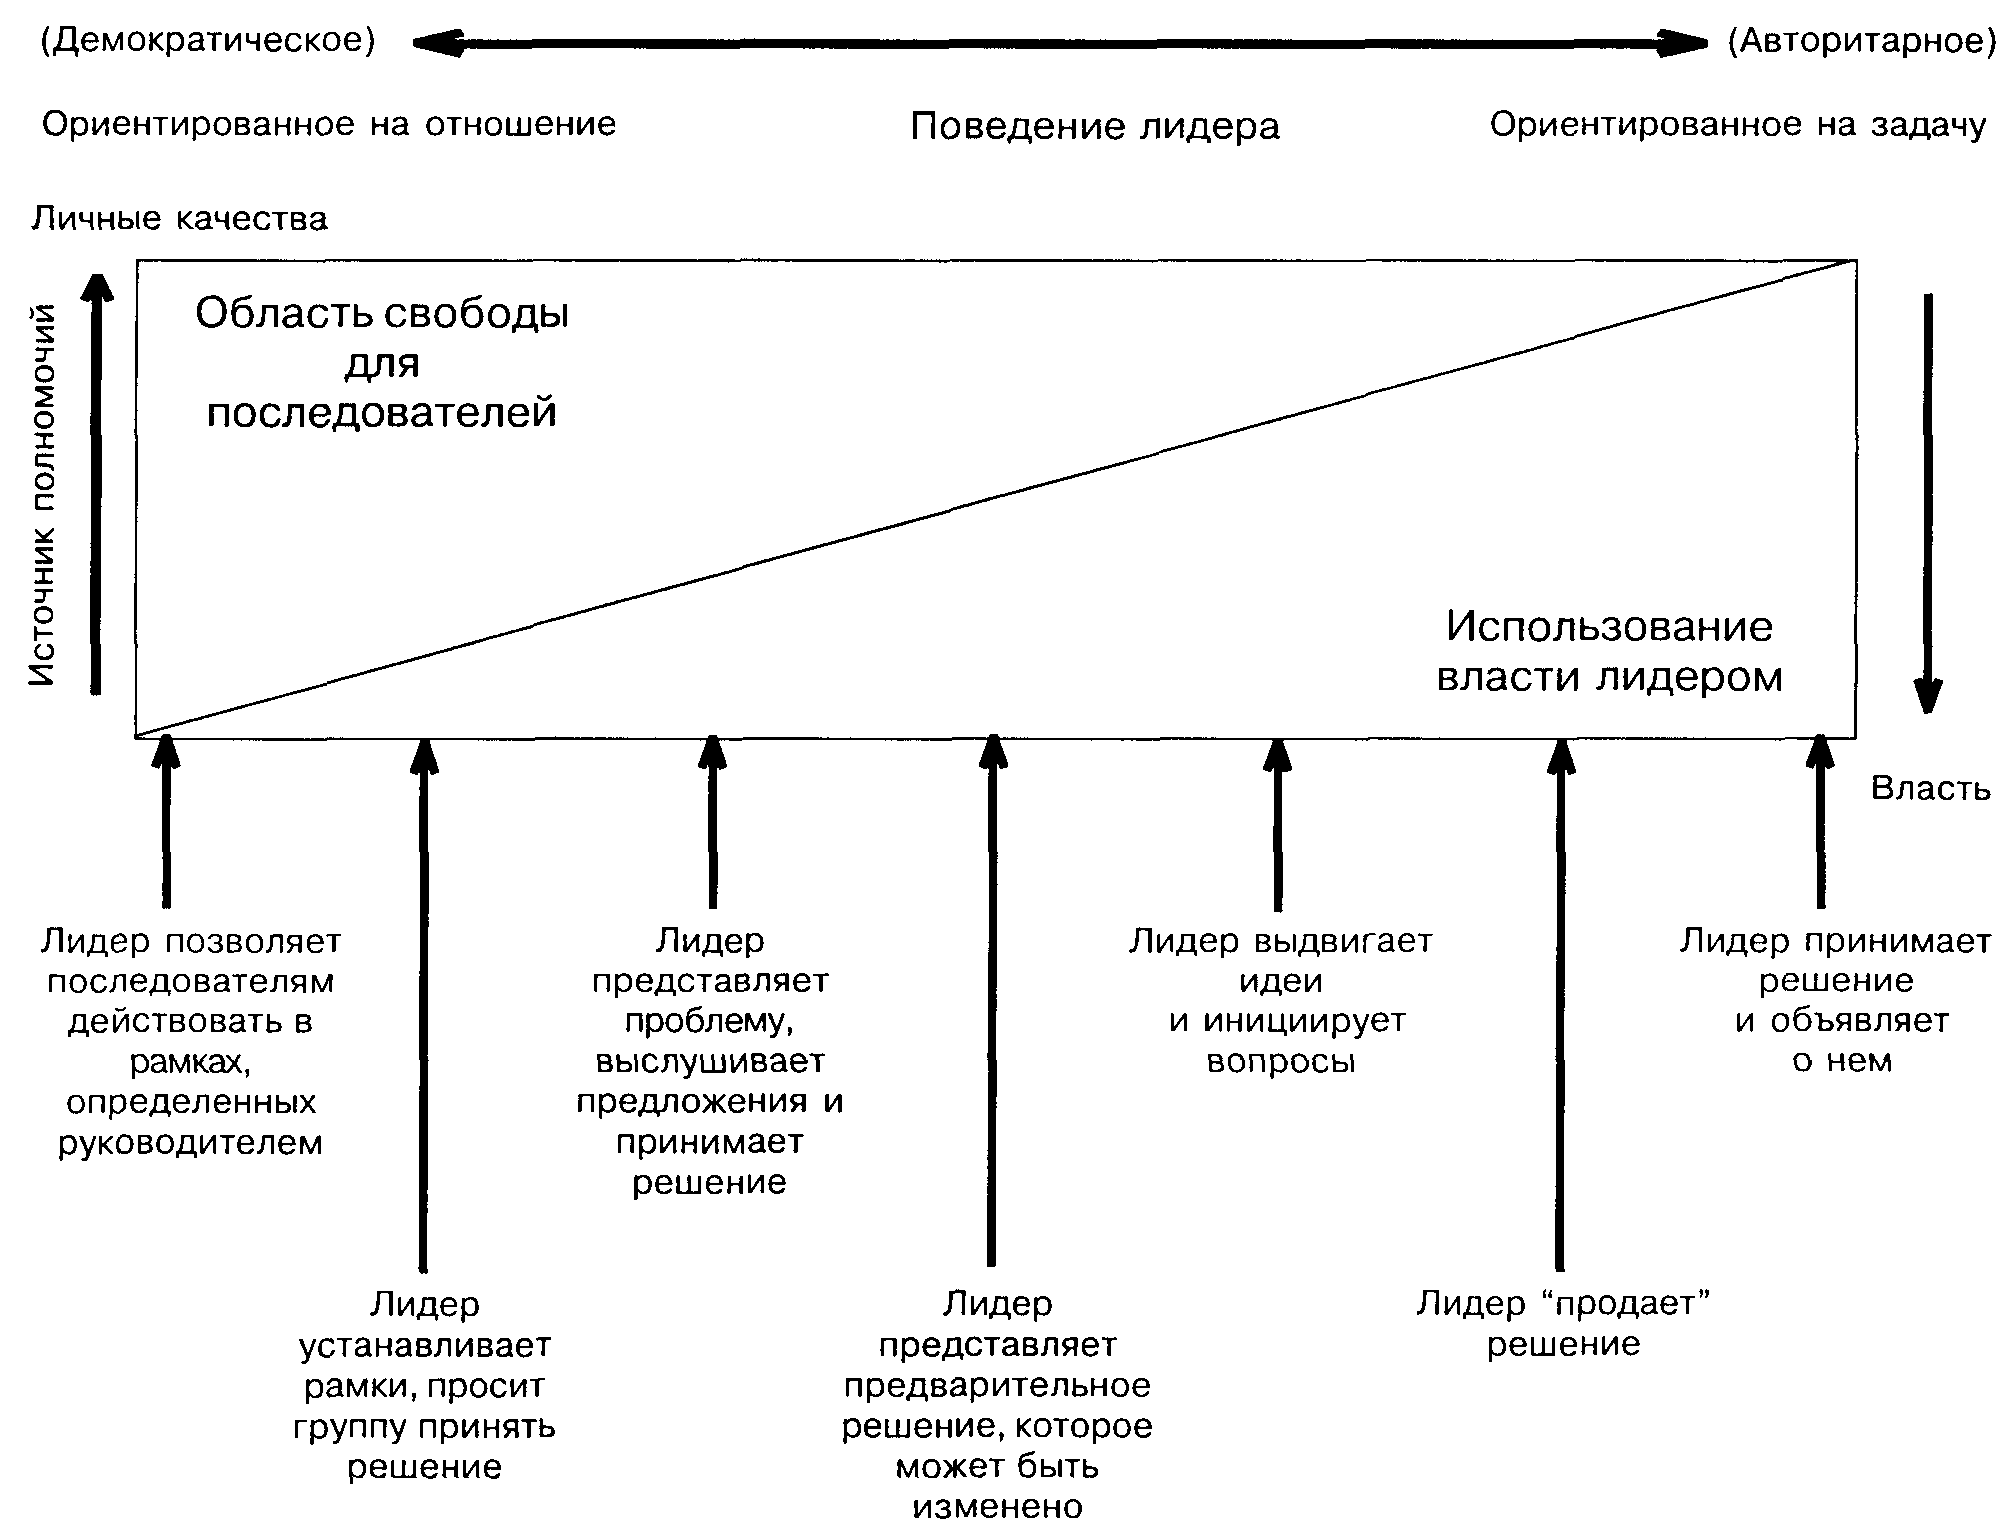
\includegraphics[width=\maxwidth{\textwidth}]{management-figures/leadership_tsh}
	\caption{Континуум лидерского поведения}
	\label{leadership_tsh}
\end{figure}

Различие между этими двумя крайними лидерскими стилями основано на предположениях лидера об источниках его власти и природе человека. 
Демократ полагает, что власть ему дается последователями, которых, он ведет, и что люди в своей основе обладают способностью к самоуправлению и творческой работе в условиях правильного мотивирования. 
Автократ считает, что власть дается его позицией в группе/организации и что люди внутренне ленивы и на них трудно полагаться. 
В первом случае имеется возможность, участия в управлении, во втором - цели, средства и политику определяет сам лидер.

\subsubsection{Модель лидерства <<путь-цель>> Хауза и Митчелла}
% http://infomanagement.ru/lekciya/model_liderstva
Рассматриваемая модель ситуационного лидерства получила своё развитие в 70-е годы. 
В своей основе она базируется на мотивационной теории ожидания. 
Исходной посылкой является предположение, что работники удовлетворены производительны тогда, когда имеется жесткая связь между и усилиями, и результатами работы, а также между результатом работы и вознаграждением. 
Отсюда модель получила свое название.
Существует прямая связь между уровнем лидерской эффективности уровнем мотивационной силы ожиданий, имеющихся последователей. 
Идеальным является вариант, когда вознаграждение полностью соответствует результату. 
Модель констатирует, что эффективный лидер --- это тот, кто помогает подчиненным идти путем ведущим к желаемой цели. 
При этом предлагаются различные варианты поведения лидера в зависимости от ситуации.

\begin{figure}[h]
	\centering
	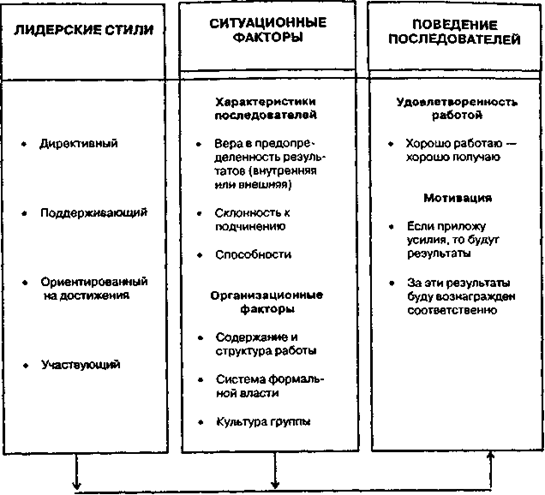
\includegraphics[width=\maxwidth{\textwidth}]{management-figures/leadership_wg}
	\caption{Модель лидерства <<путь-цель>> Хауза и Митчелла}
\end{figure}
\begin{itemize}
	\item Директивное лидерство --- высокий уровень структурирования работы, объяснение подчиненным, что и как делать, а также что и когда от них ожидается.
	\item Поддерживающее лидерство --- большое внимание нуждам работников и их благополучию, развитие дружественного рабочего климата и обращение с подчиненными как с равными.
	\item Ориентированное на достижение --- установление напряженных, но притягательных целей, огромное внимание качеству во всем, уверенность в возможностях и способностях подчиненных достичь высокого уровня выполнения работы.
	\item Участвующее лидерство --- совет с подчиненными и внимание к их предложениям и замечаниям в ходе принятия решений, привлечение подчиненных к участию в управлении.
\end{itemize}	

В отличие от концепции Фидлера, данная модель предполагает, что лидеры могут менять свое поведение и проявлять один или все из указанных стилей. 
Согласно модели, эффективная комбинация лидерских стилей зависит от ситуации.

Для анализа ситуации в модели предлагаются два типа ситуационных факторов: характеристики последователей и факторы организационной среды. 
Для описания характеристик последователей и выбора того или иного лидерского стиля используются следующие параметры:
\begin{enumerate}
	\item Вера в предопределенность происходящего от действий индивида. \\
	Выделяются два типа поведения подчиненных:
	\begin{itemize}
		\item люди внутренне уверены, что полученное вознаграждение определялось их усилиями;
		\item люди считают, что размер полученного вознаграждения контролировался внешними силами.
	\end{itemize}
	Первые предпочитают участвующий стиль лидерства, а вторые более удовлетворены директивным стилем.
	\item Склонность к подчинению. \\
	Данный параметр связан с наличием у индивида желания быть руководимым, внутренне соглашаться с влиянием других. 
	Те, кому присуще это, предпочитают в большей степени директивный стиль. 
	Другие стремятся активнее участвовать в управлении.
	\item Способности. \\ 
	Способности и имеющийся у последователей опыт определяют, насколько успешно они могут работать с лидером, ориентированным на достижение, или с лидером, привлекающим их к участию в управлении.
\end{enumerate}

В модели выделяются следующие факторы организационной среды, влияющие на выбор соответствующего лидерского стиля:
\begin{itemize}
	\item содержание и структура работы;
	\item формальная система власти в организации;
	\item групповая динамика и нормы.
\end{itemize}

Эти три фактора могут влиять на эффективность выбранного лидерского стиля в различных направлениях. 
Так, высоко структурированное задание не требует от лидера быть крайне директивным в управлении. 
Вместе с тем в организации с жесткой иерархией власти директивный лидер более эффективен, чем лидер, стремящийся привлечь подчиненных к участию в управлении. 
Забота лидера о нуждах подчиненных будет выглядеть несколько искусственно в группе с высокой степенью сплоченности. 
В целом в рамках того или иного лидерского стиля происходит взаимодействие между характеристиками последователей и организационными факторами, оказывающее влияние на восприятие мотивации последователями. 
В свою очередь восприятие, последователями, ситуации и уровень мотивации последователей определяют их удовлетворенность работой, уровень выполнения работы и признание лидера.

\subsubsection{Модель ситуационного лидерства Стинсона-Джонсона}
% http://infomanagement.ru/lekciya/model_situatsionnogo_liderstva_stinsona_jonsona
Данная модель исходит из того, что зависимость между поведением лидера и структурой работы задания является более сложной, чем это представлено в модели <<путь-цель>>. 
Модель констатирует, что хотя интерес к отношениям со стороны лидера более важен в случае, когда последователи выполняют высокоструктурированную работу, уровень интереса к работе при этом должен определяться лидером как в зависимости от характеристик последователей, так и характера самой работы, выполняемой ими.

Согласно модели, высокий интерес к работе со стороны лидера эффективен в следующих двух ситуациях:
\begin{itemize}
	\item работа высоко структурирована и последователи имеют сильную потребность в достижении и независимости. 
	При этом они обладают большими знаниями и опытом, чем им необходимо для выполнения работы;
	\item работа не структурирована, и последователи не испытывают потребности в достижении и независимости. 
	К тому же их знания и опыт ниже необходимого уровня.
\end{itemize}

Низкий интерес к работе эффективен для лидера в следующих двух ситуациях:
\begin{itemize}
	\item работа высоко структурирована и последователи испытывают потребности в достижении и независимости при наличии у них, достаточных знаний и опыта для выполнения данной работы;
	\item работа не структурирована, и последователи имеют сильную потребность в достижении и независимости при наличии у них больших знаний и опыта для выполнения данной работы. 
\end{itemize}

В табл.~\ref{tab:leadership_sj} показано поведение лидера в различных комбинациях структурированности работы и возможностей последователей. 
Модель убеждает ее пользователей, что характеристики последователей (их потребность в достижении и независимости, и их уровень знаний и опыта) являются критическими при выборе лидером эффективного стиля.

\begin{table}[h]
	\begin{tabularx}{\textwidth}{|X|X|X|}
		\hline
		& \multicolumn{2}{|c|}{Структурированность работы} \\ \hline
		& Низкая & Высокая \\ \hline 
		Возможности последователей --- высокие & Низкий интерес к отношениям и низкий интерес к работе & Высокий интерес к отношениям и высокий интерес к работе \\ \hline
		Возможности последователей --- низкие & Высокий интерес к работе и низкий интерес к отношениям & Высокий интерес к отношениям и низкий интерес к работе \\ \hline
	\end{tabularx}
	\caption{Выбор лидерского стиля в зависимости от ситуации}
	\label{tab:leadership_sj}
\end{table}

\subsubsection{Модель ситуационного лидерства Фидлера}
% http://infomanagement.ru/lekciya/model_situatsionnogo_liderstva_fidlera
Для измерения и определения лидерского стиля Фидлер предложил использовать разработанную им шкалу характеристик наименее предпочитаемого работника (НПР). 
В соответствии с этой шкалой. 
Респонденты должны, отмечать баллы по каждой из позиций шкалы, описать гипотетичесую личность, с которой они могли бы работать наименее успешно.

После того, как баллы подсчитаны по всем позициям шкалы, определяется стиль лидера.
Так, лидеры-респонденты, набравшие более высокие баллы, т.е. описавшие своего НПР очень позитивно, обладают стилем, ориентированным на отношения, а набравшие более низкие баллы имеют стиль, ориентированный на работу. 
Соответственно, эти два типа лидеров получили название лидер с высоким НПР и лидер с низким НПР. 
Согласно выводам Фидлера, лидерский стиль остается относительно постоянным и почти не меняется от ситуации к ситуации, так как в стиле отражены основы мотивации индивида: мотивированность на отношения и мотивированность на работу.

Степень контроля ситуации определяется в модели следующими тремя переменными:
\begin{enumerate}
	\item Отношения <<лидер-последователь>>. \\
	Данная переменная отражает уровень лояльности, доверительности, поддержки и уважения, испытываемых и проявляемых последователем по отношению к лидеру.
	Речь идет о признании лидера последователями, что является наиболее важным условием обретения контроля над ситуацией. 
	Приняв лидера, последователи будут делать все возможное для достижения поставленных им целей.
	\item Структурированность работы. \\
	Эта переменная отражает уровень структурированности решаемых группой проблем или выполняемых ею заданий и измеряется посредством следующих составляющих:
	\begin{itemize}
		\item ясность цели --- степень, с которой проблема или задание четко сформулированы или поставлены и знакомы исполнителям;
		\item множественность средств по достижению цели, степень возможности использования различных способов и путей. достижения цели, обоснованность решения --- степень <<правильности>> решения, подтверждаемая уровнем его принятия, его логикой или результатами.
	\end{itemize}
	Поскольку высокоструктурированная работа сама по себе содержит указания, что и как делать, то лидер получает в данной ситуации больший контроль над исполнителями.
	\item Должностная власть. \\
	Рассматриваемая переменная отражает уровень формальной власти лидера, получаемой им на основе занимаемой в организации позиции, в частности, достаточность формальной власти для того, чтобы адекватно вознаграждать или, наказывать подчиненных, повышать их в должности или увольнять.
\end{enumerate}

На рис.~\ref{leadership_fd_var} приведена принципиальная схема взаимодействия лидерского стиля с ситуационными переменными.

\begin{figure}[h]
	\centering
	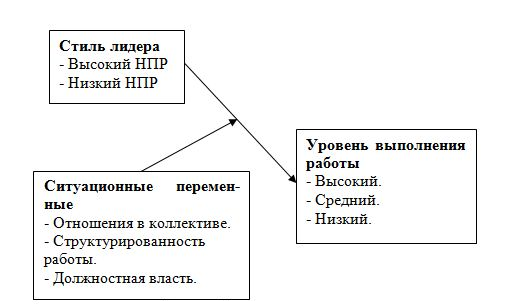
\includegraphics[width=\maxwidth{\textwidth}]{management-figures/leadership_fd_var}
	\caption{Переменные ситуационной модели Фидлера}
	\label{leadership_fd_var}
\end{figure}

Модель эффективного лидерства строится на том, что лидерство ситуационно. 
Три ситуационные переменные в сочетании с двумя лидерскими стилями дают восемь типов ситуаций (рис.~\ref{leadership_fd}), наглядно описывающих модель Фидлера.

\begin{figure}[h]
	\centering
	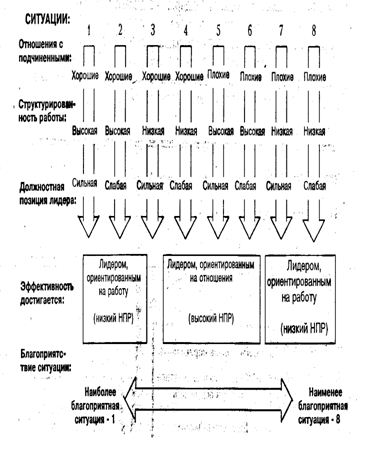
\includegraphics[width=\maxwidth{\textwidth}]{management-figures/leadership_fd}
	\caption{Типы ситуаций при использовании различных типов лидерства}
	\label{leadership_fd}
\end{figure}

\subsubsection{Модель ситуационного лидерства Херсея и Бланшарда}
% http://infomanagement.ru/lekciya/model_situatsionnogo_liderstva_herseya_i_blansharda
Данная модель равно как и другие концепции ситуационного лидерства, не предполагает поиска одного единственно верного пути для достижения эффективного лидерства. 
Вместо этого она делает упор на ситуационность лидерской эффективности. 
Одним из ключевых факторов ситуационности модель называет зрелость последователей, которая определяется степенью наличия у людей способностей и желания выполнять поставленную лидером задачу. 
Зрелость включает две составляющие: 
\begin{enumerate}
	\item Профессиональная --- это знания, умения и навыки, опыт, способности в целом. 
	Высокий уровень этой составляющей означает, что последователь не нуждается в директивах и указаниях.
	\item Психологическая зрелость --- соответствует желанию выполнять работу или мотивированности работника. 
	Высокий уровень этой составляющей у последователей не требует от лидера больших усилий по воодушевлению первых к работе, так как они уже внутренне замотивированы.
\end{enumerate}

Авторами модели были выделены четыре стадии зрелости последователей:
\begin{description}
	\item[М1] Люди не способны и не желают работать. 
	Они либо некомпетентны, либо не уверены в себе.
	\item[М2] Люди не способны, но желают работать. 
	У них есть мотивация, но нет навыков и умений.
	\item[М3] Люди способны, но не желают работать. 
	Их не привлекает то, что предлагает руководитель.
	\item[М4] Люди способны и желают делать то, что предлагает им лидер.
\end{description}

В зависимости от степени зрелости последователей лидер должен корректировать свои действия, относящиеся к установлению отношений с подчиненными и по структурированию самой работы. 
Таким образом,, модель строится на определении лидером соответствующих сложившейся ситуации уровней для поведения в области отношений \textit{(поддержка последователей)} и для поведения, относящегося к работе \textit{(директивность)}.

Поведение в области отношений связано с необходимостью для лидера больше прислушиваться к подчиненным, оказывать им поддержку, воодушевлять их и привлекать к участию в управлении. 
Поведение, относящееся к работе требует от лидера, проведения разъяснительной работы с последователями по поводу того, что и как они должны делать для того, чтобы выполнить поставленную перед ними задачу. 
Лидеры, ориентированные на такое поведение, структурируют, контролируют и внимательно следят за тем, как подчиненные работают. 
Сочетание этих двух типов лидерского поведения позволило в рамках данной модели выделить четыре основных лидерских стиля, каждый из которых наиболее соответствует определенной степени зрелости последователей:
\begin{enumerate}
	\item Указывающий стиль (S1) является лучшим в случае низкой зрелости последователей. 
	Лидер вынужден проявлять высокую директивность и тщательный присмотр за работниками, помогая таким образом людям, не способным и не желающим взять на себя ответственность по работе, устранить-неуверенность в том, что работа будет закончена.
	\item Убеждающий стиль (S2) является лучшим для использования в условиях умеренно низкой зрелости последователей, реализуя в равной мере директивность и поддержку тем, кто не способен, но желает работать. 
	Руководитель, использующий этот стиль, помогает им путем объяснения и вселяет в них уверенность в возможности выполнения задания.
	\item Участвующий стиль (S3) является лучшим при умеренно высокой зрелости последователей. 
	Способные к работе, но не желающие ее выполнять, подчиненные нуждаются в партнерстве со стороны лидера, чтобы быть более мотивированными на выполнение работы. 
	Предоставляя таким людям возможность участвовать в принятии решений на своем уровне, руководитель использует данный стиль, чтобы вызвать у последователей желание выполнять задание.
	\item Делегирующий стиль (S4) является лучшим для руководства высоко-зрелыми последователями. 
	Стиль характеризуется незначительной директивностью и поддержкой работников. 
	Это позволяет последователям, способным и желающим работать, взять на себя максимум ответственности за выполнение задания. 
	Данный лидерский стиль способствует развитию творческого подхода к работе.
\end{enumerate}

\begin{figure}[h]
	\centering
	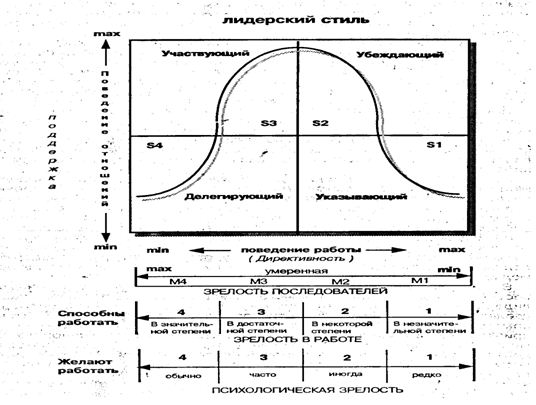
\includegraphics[width=\maxwidth{\textwidth}]{management-figures/leadership_hb}
	\caption{Модель ситуационного лидерства Херсея и Бланшарда}
\end{figure}

\subsubsection{Ситуационная модель принятия решений Врума-Йеттона-Яго}
% http://infomanagement.ru/lekciya/situatsionnaya_model
Одной из наиболее современных в объяснении ситуационного лидерства является модель, предложенная Виктором Врумом и Филиппом Йеттоном, которая позже была существенно дополнена с участием Артура Яго. 
Аналогично модели <<путь-цель>>, данная модель предлагает определять эффективный лидерский стиль в зависимости от ситуации. 
Предполагается также, что один и тот же лидер может использовать различные стили. 

Основным отличием модели является ее ориентированность только на один аспект лидерского поведения --- привлечение подчиненных к участию в принятии решений.
Соответственно лидеру предлагается концентрировать внимание на проблеме, которая должна быть решена, и на ситуации, в которой проблема возникла.
Подразумевается также, что ряд социальных процессов может оказать влияние на уровень участия подчиненных в решении проблем.

Главной идеей модели является то, что степень или уровень привлечения подчиненных к участию в принятии решения зависит от характеристик ситуации. 
В соответствии с моделью не существует одного единственно верного способа принятия решения, пригодного для всех ситуаций. 
После анализа и оценки каждого аспекта проблемы лидер определяет, какой стиль, с точки зрения участия подчиненных в принятии решения, ему лучше использовать.
В рассматриваемой модели эффективность решения $P_\textup{эфф}$ определяется на основе уравнения, показывающего, что она зависит от качества решения $P_\textup{кач}$ и уровня принимаемых подчиненными обязательств по выполнению решения $P_\textup{обяз}$, а также от степени срочности решения $P_\textup{время}$. 
Предпосылкой модели является представление, что отведенное ситуацией для решения время наряду с остальными двумя является, критическим фактором. 
Ситуация, в которой ограничение времени не играет роли, определяет этот показатель на нулевом уровне.
\[
P_\textup{эфф} = P_\textup{кач} + P_\textup{обяз} - P_\textup{время}
\]

Полная критериальная основа <<общей эффективности решения>> $O_\textup{эфф}$ предполагает учет в ней факторов <<стоимости>> и <<развития>>.
\[
O_\textup{эфф} = P_\textup{эфф} - \textup{стоимость} - \textup{развитие}
\]

В приведенной формуле показатель <<стоимость>> означает потерянное из-за решения время, которое в другом случае могло, принести больше пользы. 
Показатель <<развитие>> отражает тот выигрыш, который получен за пределами единолично принятого решения.

Последний разработанный вариант модели предлагает использование дерева решений для определения лидерского стиля, наиболее соответствующего сложившейся ситуации. 
При использовании модели менеджер как бы следует по ветвям этого дерева слева направо. 
Делая это он сталкивается с 10 проблемными ситуациями. 
Оценка ситуаций делается им по 8 аспектам проблемы с выбором по каждому из них ответа: высокий/высокая или низкий/низкая. 
Эти ответы выводят менеджера в конце концов на конкретную проблемную ситуацию и рекомендуемый для, нее стиль принятия решения (рис.~\ref{leadership_vyy_1}).

\begin{figure}[h]
	\centering
	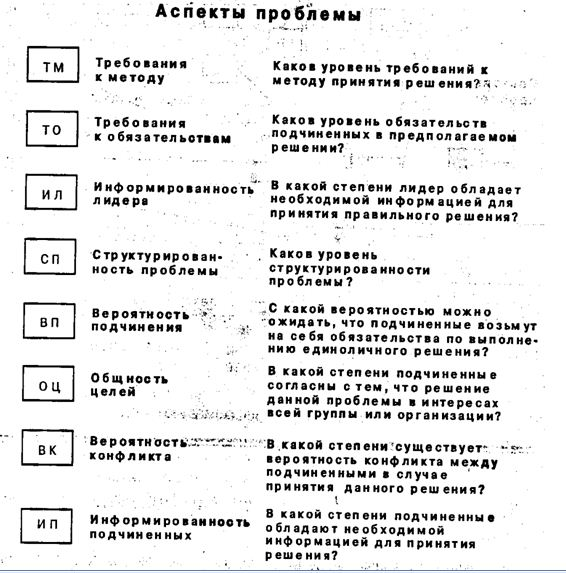
\includegraphics[width=\maxwidth{\textwidth}]{management-figures/leadership_vyy_1}
	\caption{Аспекты проблемы}
	\label{leadership_vyy_1}
\end{figure}

Для принятия решений в модели в зависимости от ситуации и степени привлечения подчиненных предлагается использовать пять стилей: 
\begin{description}
	\item[AI] Руководитель принимает решение сам, используя имеющуюся у него на данное время информацию.
	\item[АII] Руководитель получает необходимую информацию от своих подчиненных и затем сам принимает решение. 
	Работники привлекаются только на этапе сбора информации. 
	Выработку решения и его принятие осуществляет руководитель.
	\item[КI] Руководитель на индивидуальной основе делится соображениями по проблеме с имеющими к ней отношение подчиненными с целью получения от них идей и предложении, не собирая при этом их в группу. 
	Затем он сам принимает решение, которое может основываться на вкладе подчиненных, а может и нет.
	\item[КII] Руководитель делится соображениями по проблеме с подчиненными, собрав их вместе. 
	В ходе совещания он собирает их идеи и предложения. 
	Затем он принимает решение, которое может либо отражать, либо не отражать их вклад.
	\item[ГII] Руководитель делится соображениями по проблеме с оценивают альтернативы и пытаются достичь консенсуса относительно решения. 
	Роль, выполняемая при этом руководителем, больше похожа на роль председателя собрания, координирующего дискуссию. 
	Концентрирующего внимание на проблеме и делающего все для того, чтобы рассматривались наиболее важные аспекты проблемы. 
	Руководитель не пытается влиять на группу с тем, чтобы она приняла его решение, и проявляет готовность принять и выполнить любое решение, получившее поддержку всей группы. 
\end{description}

Одной из отличительных особенностей модели является то, что в целом она делает больший упор на изучение ситуации, чем на изучение личности лидера.
Действительно, может быть, имеет больше смысла говорить об автократической ситуации и ситуации участия, чем об автократическом лидере или участвующем лидере.

\begin{figure}[h]
	\centering
	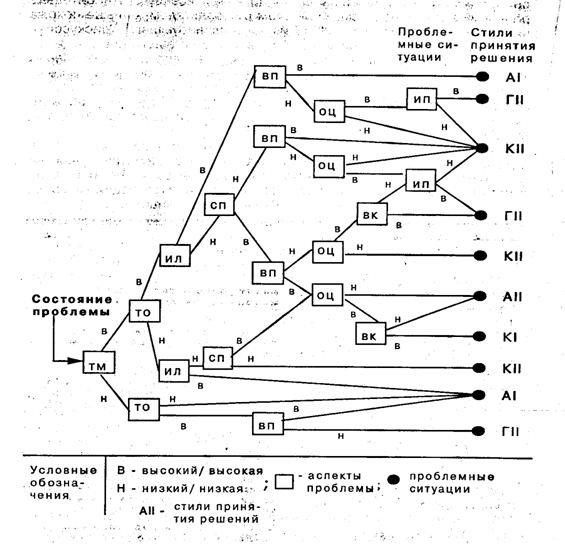
\includegraphics[width=\maxwidth{\textwidth}]{management-figures/leadership_vyy_2}
	\caption{Дерево решений Врума-Яго}
	\label{leadership_vyy_2}
\end{figure}

\subsection{Новое в теориях лидерства}
\subsubsection{Атрибутивное лидерство}
Концепция атрибутивного лидерства основана на причинно-следственных связях между тем, что произошло и тем, что люди считают причиной произошедшего. 
Такую связь объясняет теория атрубуции. 
Атрибутивный подход исходит из того, что выбор лидера, в равной мере, как и поведение последователей, обусловлены реакцией лидера на поведение последних.
Наблюдая за работой сотрудников, лидер получает информацию о том, как она выполняется. 
В зависимости от этого он делает выводы о поведении каждого работника и корректирует стиль своего поведения таким образом, чтобы адекватно реагировать на действия подчиненного. 

Атрибутивное лидерство пытается ответить на вопрос, почему люди ведут себя так, а не иначе. 
Определение лидером причин поведения последователя базируется на трех признаках: личность, сама работа, организационное окружение или обстоятельства.

В поиске причин лидер пытается получить три вида информации о поведении последователей:
\begin{enumerate}
	\item Степень отличия задания. \\
	Это связано с желанием лидера понять связь между поведением и работой с той точки зрения, насколько определенное поведение может быть вызвано отличительными особенностями задания. 
	\item Последовательность поведения работника. \\ 
	Лидера интересует то, насколько подчиненный последователен в проявлении данного поведения или как часто это поведение у него повторяется.
	\item Степень уникальности поведения. \\
	Лидер учитывает, насколько другие подчиненные ведут себя таким же образом, т.е. является ли данное поведение уникальным, характерным для одного подчиненного или наблюдается у всей группы. 
\end{enumerate}

Технология развития данного лидерства сосредоточена на двух задачах:
\begin{itemize}
	\item создание (поддержание) харизматического образа какого-либо человека;
	\item формирование его отношений с последователями. 
\end{itemize}

\subsubsection{Харизматическое лидерство}
Харизма --- одаренность человека, его исключительность. 
Харизматическим считается лидер, который способен оказывать глубокое воздействие на последователей в силу своих личностных качеств. 
В целом харизматическому лидеру приписывают уверенность в себе, стремление к власти, убежденность в совей правоте, нестандартное видение решения проблемы, умение обосновать его перед последователями и побудить их к действию, неординарное поведение при реализации своего видения. 
Присущая такому человеку жажда деятельности передается другим людям, и они искренне верят в прирожденную способность к лидерству. 

Значение харизматического лидерства для бизнеса возрастает по мере необходимости проведения в организации радикальных изменений. 
В стабильной ситуации оно не всегда эффективно. 

\subsubsection{Преобразующее лидерство} 
Это лидерство эффективно в ситуациях изменений, динамического развития, реинжиниринга бизнес-процессов. 

Лидер-реформатор мотивирует последователей путем:
\begin{itemize}
	\item повышения уровня их сознательности в восприятии поставленной цели;
	\item предоставления им возможности соотношения своих личных интересов с общей целью;
	\item создания атмосферы доверительности и убеждения последователей в необходимости саморазвития. 
\end{itemize}

Лидер-реформатор --- это новатор, стратег-преобразователь, а не спаситель, его цель не изменить мир, а адаптироваться в нем через развитие персонала, организационное развитие. 
Модель преобразующего лидерства предполагает наличие у лидера последователей определенного поведения, которое наиболее подходит для творческого решения проблемы в кризисной ситуации.

\subsection{Природа конфликта и стресса}
Конфликт --- это отсутствие согласия между двумя и более сторонами, которыми могут быть как конкретные лица, группы, так и организации в целом, причем это несогласие между сторонами приводит к тому, что сознательное поведение одной из сторон вступает в противоречие с интересами другой стороны.

Причины: распределение ресурсов, взаимозависимость задач, различие в целях, различие в представлениях и ценностях, различие в манерах поведения и жизненном опыте и неудовлетворительных коммуникациях.

Типы конфликтов:
\begin{itemize}
	\item внутриличностный;
	\item межличностный;
	\item между личностью и группой;
	\item внешний.
\end{itemize}

Позитивные функции конфликта.
\begin{itemize}
	\item разрядка напряженности между сторонами;
	\item сплочение коллектива перед внешним врагом. Широко известно, что дружить легче против кого-то;
	\item несомненно, внешний враг может помочь усилению консолидации членов группы;
	\item получение новой информации об оппоненте и окружающей социальной среде;
	\item большая расположенность к сотрудничеству в будущем;
	\item снятие синдрома покорности у подчиненных.
\end{itemize}

Негативные функции конфликта.
\begin{itemize}
	\item большие эмоциональные и материальные затраты на участие в конфликте;
	\item рост неудовлетворенности, плохое моральное состояние;
	\item снижение производительности труда, рост текучести кадров;
	\item представление о второй стороне как о враге;
	\item уменьшение сотрудничества после завершения конфликта;
	\item сложное восстановление деловых отношений (<<шлейф>> конфликта);
	\item усиление тенденции к авторитарному руководству.
\end{itemize}

\subsection{Управление конфликтной ситуацией}
% http://www.nnre.ru/delovaja_literatura/menedzhment_konspekt_lekcii/p12.php
Управление конфликтом --- это целенаправленное воздействие на устранение причин конфликта или на коррекцию поведения участников. 
Методы управления и разрешения конфликтов делятся на три группы: внутриличностные, структурные и межличностные.

Внутриличностные методы воздействуют на отдельную личность и состоят в правильной организации своего собственного поведения, в умении высказывать свою точку зрения, не вызывая защитной реакции со стороны оппонента.

Структурные методы изменяют структуру заданий работникам или структуру организации. К структурным методам разрешения конфликтов относятся следующие:
\begin{enumerate}
	\item Разъяснение требований к работе. 
	\item Использование координационных и интеграционных механизмов, которые улучшают согласованность между подразделениями и отдельными людьми.
	\item Постановка общеорганизационных целей.
	\item Использование системы вознаграждений для поощрения поведения, направленного на избежание негативных последствий конфликтов.
\end{enumerate}

Методы разрешения межличностных конфликтов через сотрудничество:
\begin{enumerate}
	\item Определите проблему в категориях целей, а не решений.
	\item После того, как проблема определена, определите решения, которые приемлемы для обеих сторон.
	\item Сосредоточьте внимание на проблеме, а не на личных качествах другой стороны.
	\item Создайте атмосферу доверия, увеличив взаимное влияние и обмен информацией.
	\item Во время общения создайте положительное отношение друг к другу, проявляя симпатию и выслушивая мнения другой стороны, а также сводя к минимуму проявления гнева и угроз.
\end{enumerate}

\subsection{Управление изменениями}
Управление изменениями --- это структурный подход к переводу индивидов, команд и организаций из текущего состояния в желаемое будущее состояние. 
Целью этого организационного процесса является расширение прав и возможностей сотрудников принять и поддержать изменения в их текущем бизнес-окружении. 
В управлении проектами, управление изменениями рассматривается как процесс управления проектом, в котором формально представлены и одобрены изменения проекта.

В управлении изменениями используются различные подходы для анализа, подготовки и проведения изменений:
\begin{enumerate}
	\item Индивидуальные изменения.
	\item Командные изменения.
	\item Организационные изменения.
\end{enumerate}

Использование типовых шагов для проведения изменений подробно рассмотрено в работах Коттера, таких как:
\begin{enumerate}
	\item Преодоление состояния удовлетворенности текущей ситуацией.
	\item Формирование команды для проведения изменения.
	\item Определение видения желаемого будущего и стратегии перехода.
	\item Широкое информирование о проводимых изменениях.
	\item Устранение препятствий и барьеров, мешающих проведению изменений.
	\item Достижение быстрых первых успехов.
	\item Поддержание процесса изменений с целью недопущения отката назад.
	\item Закрепление проведенных изменений в корпоративной культуре.
\end{enumerate}

Управление изменениями оперирует такими понятиями, как лидерство, эффективность коммуникаций и принятие потребности в изменениях для разработки точных стратегий перехода, для того чтобы преодолеть неизбежное сопротивление переменам.

\subsection{Сущность, функции и элементы маркетинга}
Маркетинг --- это комплексная система организации производства и сбыта, ориентированная на возможное более полное удовлетворение быстро меняющихся и все более разнообразных потребностей потребителей посредством рынка и получение на этой основе устойчивой прибыли и конкурентных преимуществ.

Выделяют 3 (три) подхода к определению сущности маркетинга:
\begin{itemize}
	\item как самостоятельный вид производственной деятельности;
	\item как функция управления;
	\item как современное видение философии бизнеса.
\end{itemize}

Концепция маркетинга --- это философия управления, которая способствует получению товара производителями прибыли посредством удовлетворения потребностей потребителей.

% http://www.grandars.ru/student/marketing/funkcii-marketinga.html
Главные функции маркетинга:
\begin{itemize}
	\item аналитическая функция;
	\item продуктово-производственная функция;
	\item сбытовая функция (функция продаж);
	\item функция управления и контроля.
\end{itemize}

Комплекс маркетинга --- совокупность управляемых элементов маркетинговой деятельности организации, манипулируя которыми она старается наилучшим образом удовлетворить потребности целевых рынков.
% https://ru.wikipedia.org/wiki/%D0%A2%D0%B5%D0%BE%D1%80%D0%B8%D1%8F_4P
Теория 4P \textit{(маркетинг-микс)} — маркетинговая теория, основанная на четырёх основных <<координатах>> маркетингового планирования:
\begin{description}
	\item[Product] Товар или услуга, ассортимент, качество, свойства товара, дизайн и эргономика.
	\item[Price] Цена, наценки, скидки.
	\item[Promotion] Продвижение, реклама, пиар, стимулирование сбыта.
	\item[Place] Месторасположения торговой точки, каналы распределения, персонал продавца.
\end{description}

\subsection{Задачи, виды и структура маркетинговых исследований}
Маркетинговое исследование --- это систематический поиск, сбор, анализ и представление данных и сведений, относящихся к конкретной рыночной ситуации, с которой пришлось столкнуться предприятию. 
Маркетинговое исследование можно также определить как систематический сбор, учет и анализ данных по маркетингу и маркетинговым проблемам в целях совершенствования качества процедур принятия решений и контроля в маркетинговой среде. 
Имеется целый ряд аналогичных и иных определений маркетинговых исследований.

Основные цели маркетингового исследования:
\begin{itemize}
	\item уменьшить неопределенность и минимизировать риск в процессе принятия управленческих решений;
	\item следить за процессом реализации маркетинговых задач.
\end{itemize}

Глобальные цели маркетингового исследования --- это информационное обеспечение маркетинга, то есть сбор необходимой информации и аналитическое обеспечение, заключающееся в использовании математических моделей для анализа данных и получения с их помощью прогнозов и возможности принятия оптимальных решений.

% http://works.doklad.ru/view/hARiKdLaWJM.html
Задачи маркетинговых исследований могут быть самыми разнообразными и диктоваться потребностями разработки стратегии маркетинга, формирование ценовой, товарной, коммуникационной, сбытовой политики и другими аспектами управления маркетингом на предприятии. 
Наиболее типичные решаемые задачи маркетинговых исследований:
\begin{itemize}
	\item изучение характеристик рынка;
	\item замеры потенциальных возможностей рынка;
	\item анализ распределения долей рынка между фирмами;
	\item анализ сбыта;
	\item изучение тенденций деловой активности;
	\item изучение товаров конкурентов;
	\item краткосрочное прогнозирование;
	\item изучение реакции на новый товар и его потенциала;
	\item долгосрочное прогнозирование;
	\item изучение политики цен.
\end{itemize}

\begin{figure}[h]
	\centering
	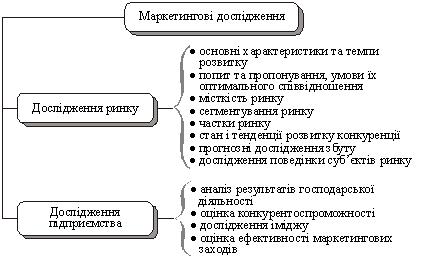
\includegraphics[width=\maxwidth{\textwidth}]{management-figures/marketing_structure}
	\caption{Структура маркетинговых исследований}
\end{figure}

Типы маркетинговых исследований:
\begin{enumerate}
	\item Разведочные или поисковые, предшествующие разработке программы основного исследования. 
	Предпринимаются для сбора предварительной информации, освещающие проблемы, позволяет выдвинуть гипотезы.
	\item Описательные \textit{(дескриптивные)}. 
	Имеющие целью констатацию реальных фактов, событий, показателей, полученных в результате сбора информации. 
	\item Экспериментальные. 
	Проводится с целью проверки выдвинутой гипотезы.
	\item Аналитические. 
	Проводимое для выявления и моделирования связи и деятельности фирмы с факторами окружающей среды. 
\end{enumerate}

\subsection{Маркетинговое сегментирование рынка}
Сегментирование рынка --- это процесс разделения рынка на отдельные части --- сегменты, отличающиеся друг от друга разными возможностями сбыта.

Сегмент рынка --- это особым образом выделенная часть рынка, группы потребителей или предприятий, обладающих определенными общими признаками. 
Может быть осуществлено по множеству критериев --- мерилам оценки обоснованности выбора сегмента рынка. 
Принцип сегментирования --- показатель выделения данного сегмента рынка. 

\begin{figure}[h]
	% http://powerbranding.ru/segmentirovanie/osnovy/
	\centering
	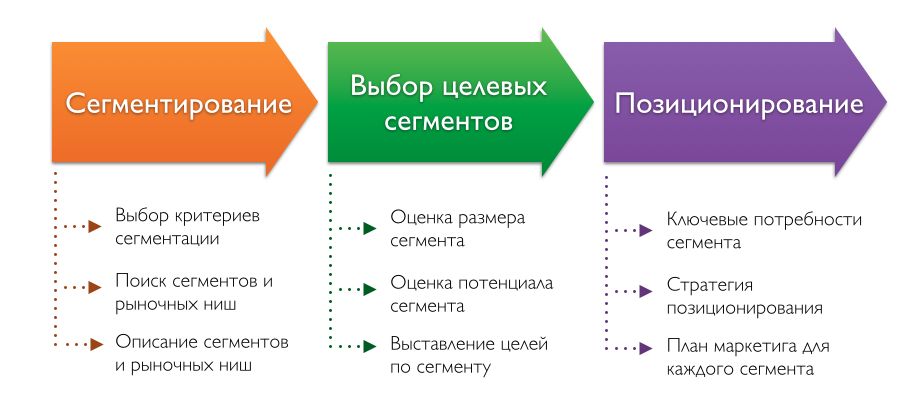
\includegraphics[width=\maxwidth{\textwidth}]{management-figures/marketing_segmentation_process}
	\caption{Схема сегментации рынка}
\end{figure}

Могут быть использованы следующие критерии:
\begin{enumerate}
	\item Различия между потребителями позволяющее объединить их в один сегмент.
	\item Сходство, формирующие устойчивость.
	\item Наличие показателей, позволяющих измерить характеристики и требования потребителей, определить емкость рынка.
	\item Возможность выстоять в конкурентной борьбе.
	\item Достаточность объема продаж.
	\item Доступность сегмента для предприятия.
\end{enumerate}

Существует три варианта охвата рынка:
\begin{itemize}
	\item недифференцированный маркетинг;
	\item дифференцированный маркетинг;
	\item концентрированный маркетинг.
\end{itemize}

На выбор стратегии охвата рынка влияют ресурсы фирмы, степень однородности продукции, этапы жизненного цикла товара, степень однородности рынка.

Обобщенные критерии правильного определения сегмента:
\begin{itemize}
\item доступность;
\item измеримость;
\item значимость по размерам, динамике спроса и своему совокупному потенциалу;
\item заметные отличия от других составных частей рынка;
\item относительная устойчивость сходства спроса со стороны потребителей.
\end{itemize}

\subsection{Цель и суть товарной политики}
Товарная политика --- это совокупность решений, касающихся формирования эффективной рыночно-ориентированной производственной программы предприятия.

Товарная политика ­­--- область целенаправленных действий по отдельным предложенным для использования товарам и услугам (вид, количество, свойство и т.д.), а также по совокупности отдельных продуктов (ширина, глубина, структура ассортимента).

Цель товарной политики --- добиться сбалансированного товарного ассортимента и конкурентоспособности каждого отдельного продукта, а так же:
\begin{itemize}
	\item обеспечение прибыли;
	\item увеличение товарооборота;
	\item увеличение доли рынка;
	\item снижение расходов на производство и маркетинг;
	\item повышение имиджа;
	\item рассеивание риска.
\end{itemize}

Задачи товарной политики --- принятие решений в области предлагаемых предприятием товаров, касающихся самих продуктов, их присутствия на рынке, а также связанных с этим решений по производственной программе.

\subsection{Использование средств стимулирования сбыта}
% http://www.aup.ru/books/m99/7_9.htm
Стимулирование сбыта --- это совокупность приемов, применяемых на протяжении всего жизненного цикла товара в отношении трех участников рынка (потребителя, оптового торговца, продавца), для краткосрочного увеличения объема сбыта, а также для увеличения числа новых покупателей.

Стимулирование сбыта имеет многоцелевую направленность: потребитель, продавец, торговый посредник.

Выбор средств стимулирования зависит от поставленных целей. 
Все средства можно объединить в три большие группы:
\begin{itemize}
	\item предложение цены (продажа по сниженным ценам, льготные купоны, талоны, дающие право на скидку);
	\item предложение в натуральной форме (премии, образцы товара);
	\item активное предложение (конкурсы покупателей, игры, лотереи).
\end{itemize}

Процесс выбора комплекса продвижения товара включает этапы:
\begin{enumerate}
	\item Определение цели продвижения. 	
	\begin{enumerate}
		\item Информирование потребителей.
		\item Стимулирование сбыта.
		\item Формирование благоприятного имиджа.
		\item Влияние на привычки потребителей.
		\item Поддержание деловых отношений, взаимопонимание с деловыми партнерами и т.д.
	\end{enumerate}
	\item Оценивание факторов, влияющих на комплекс продвижения.		
	\begin{enumerate}
		\item Цели фирмы.
		\item Стратегия.
		\item Целевая аудитория.
		\item Тип товара.
		\item Этап жизненного цикла.
		\item Объем рынка.
		\item Стоимость.
	\end{enumerate}
	\item Разработка стратегии продвижения.	
	\begin{enumerate}
		\item Интенсификация рекламы.
		\item Новая рекламная компания.
	\end{enumerate}
	\item Составление и распределение бюджета распределения.	
	\begin{enumerate}
		\item <<Снизу-вверх>>. Общая сумма затрат на комплекс продвижения.
		\item <<Сверху-вниз>>. Составляем статьи отдельно для рекламы, персональной продажи, а потом считаем общую сумму.
	\end{enumerate}
	\item Методы составления бюджета.	
	\item Оценивание комплекса продвижения.	
\end{enumerate}

\subsection{Ценовая политика в маркетинговой деятельности. Методы расчета и установления цены}
Цена --- денежное выражение стоимости товара, предназначенное для непрямого измерения общественно-необходимых затрат рабочего времени на производство товара. Количество денежных единиц, которые должен заплатить покупатель продавцу за весь товар или его единицу.

Ценовая политика --- это установление определенных цен и способов маневрирование ими в зависимости от положения на рынке, которые позволяют овладеть долю рынка, получить расчетную прибыль, а также решить другие стратегические и оперативные задачи.

На цену влияют внешние факторы (политическая стабильность страны, экономика, гос. регулирование цены, состояние рынка) и внутренний (стратегия и тактика фирмы, специфика жизненного цикла товара, особенности производства и характеристики системы продвижения товаров на рынке).

Алгоритм определение цены:
\begin{enumerate}
	\item Определение целей. 	
	\item Определение и анализ спроса. 	
	\item Анализ издержек производства. 	
	\item Анализ цен товаров конкурентов. 	
	\item Методы ценообразования. 	
	\item Выбор ценовой стратегии. 	
	\item Адаптация цен. 	
\end{enumerate}

Методы ценообразования:
\begin{itemize}
	\item ориентированный на затратах;
	\item ориентированная на спрос;
	\item ориентируемые на конкурентов.
\end{itemize}

\end{document}